\chapter{Base knowledge}

Per effettuare comunicazioni tramite internet, vi è il bisogno che tutti i dispositivi connessi rispettino determinati meccanismi; questo si rende necessario a causa dell'elevata eterogeneità derivata da hardware e software differenti.
Questi meccanismi, che prendono il nome di \textit{protocolli}, sono strutturati secondo diversi layer (livelli) formando lo stack TCP/IP.  \\
Sebbene l'idea originale (modello ISO/OSI) prevedesse un modello composto da sette livelli, de facto lo schema attualmente in uso ne prevede solamente quattro. Nonostante ciò, nella terminologia informatica la numerazione dei livelli è rimasta quella precedente.
\\
\begin{table}[htb]
	\centering
	\begin{tabular}{| l | c |}
		\hline
		Livello 7 & Applicativo
		\\
		\hline
		Livello 4 & Trasporto
		\\
		\hline
		Livello 3 & Rete
		\\
		\hline
		Livello 2 & Fisico
		\\
		\hline
		
	\end{tabular}
	\caption{Livelli dello stack TCP/IP}
	\label{tab:stack}
\end{table}

\section{Funzionamento dello stack TCP/IP}
Il meccanismo dello stack prevede che ad ogni livello vengano aggiunte al messaggio delle intestazioni (header), a partire dal layer più alto, che verranno valutate dal medesimo livello del ricevente.
Si precisa che l'ordine in cui si valutano gli header dei livelli è inverso rispetto a quello del mittente; il ricevente partirà infatti dal livello più basso.
Questa procedura prende il nome di \textit{incapsulamento} ed è riassunta nella seguente figura:


\begin{figure}[h]
	\centering
	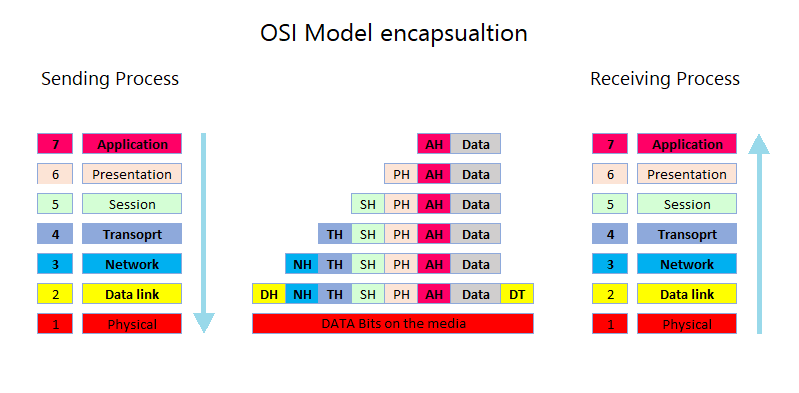
\includegraphics[width=\textwidth]{figures/incapsulamento.png}
	\caption{Incapsulamento nel modello ISO/OSI}
	\label{incapsulamento}
	\cite{incapsulamento}
\end{figure}

\section{Header per il fingerprinting}
Gli header aggiunti ad ogni livello sono formati da vari campi contententi informazioni utili per la comunicazione, e il valore che questi assumono in determinate situazioni è dipendente dal sistema operativo che si sta utilizzando.

Si prenda ad esempio l'header TCP, un protocollo del livello 4 dello stack:\\

\begin{figure}[H]
	\centering
	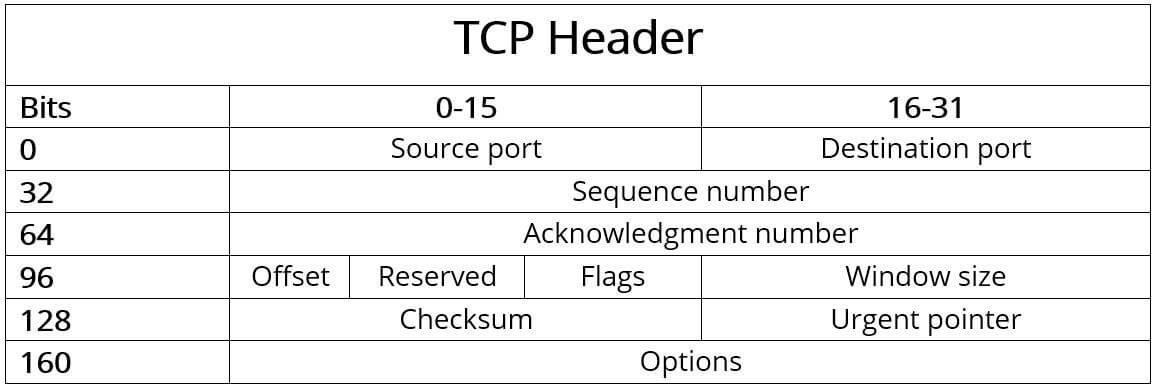
\includegraphics[width=\textwidth]{figures/headerTCP.JPG}
	\caption{Header TCP}
	\label{headerTCP}
	\cite{headerTCP}
\end{figure}

Il campo \textit{option} permette di segnalare al ricevente l'uso di alcune opzioni di comunicazione; il loro supporto e l'effettivo utilizzo, essendo queste facoltative e quindi peculiari di specifici sistemi operativi, rivestono quindi particolare importanza ai fini del fingerprinting.
Esempi analoghi si possono trovare nei protocolli ad ogni livello dello stack, e l'unione delle informazioni acquisite dall'analisi degli header consente di poter individuare con una discreta precisione il sistema operativo del dispositivo target.